\documentclass[12pt,a4paper]{article}
\usepackage[utf8]{inputenc}
\usepackage[english,russian]{babel}
\usepackage{amssymb,amsfonts,amsmath,cite,enumerate,float,indentfirst}
\usepackage{graphicx}
\usepackage{geometry}
\usepackage{systeme}
\usepackage{amsmath}
\usepackage[bottom]{footmisc}
\usepackage{hyperref}
\usepackage{url}

\hypersetup{
	colorlinks,
	citecolor=black,
	filecolor=black,
	linkcolor=black,
	urlcolor=black
}
\geometry{left=2cm}
\geometry{right=1.5cm}
\geometry{top=2cm}
\geometry{bottom=2cm}

\begin{document}
	\begin{titlepage}
		\begin{center}		
			\vfill	
			Санкт-Петербургский политехнический университет \\
			Петра Великого\\
			\vskip 1cm
			Высшая школа прикладной математики и вычислительной физики \\
			Кафедра «Прикладная математика и информатика»
			\vfill
			\textbf{Отчёт\\
				по лабораторной работе №1\\
				по дисциплине\\
				«Интервальный анализ»\\}
			\vfill
		\end{center}
		\vfill
		\hfill
		\begin{minipage}{0.4\textwidth}
			Выполнил студент:\\
			Лапотников Павел Вадимович\\
			группа: 5030102/90201\\
		\end{minipage}
		\vfill
		\hfill 
		\begin{minipage}{0.4\textwidth}
			Проверил:\\
			к.ф.-м.н., доцент\\
			Баженов Александр Николаевич\
		\end{minipage}
		\vfill
		\hfill 
		\begin{center}
			Санкт-Петербург\\2022 г.
		\end{center}
	\end{titlepage}
	
	\tableofcontents
	\listoffigures
	\pagebreak
	
	\section{Постановка задачи}
	    
	    \subsection{Постановка задачи для матрицы линейной регрессии} \label{problem:lin_reg}
    	    Во многих задачах возникает ситуация, в которой нужно выяснить неособенность матрицы. Одной из таких задач является задача в общей регрессионной постановке
    	    \begin{equation}
    	        y = X\beta
    	    \end{equation}
	    
	        Пусть число уравнений $m = 2$ и погрешность входных данных неизвестна. Пусть матрица средних значений иммеет вид
	        
	        \begin{equation}
	            midX = \begin{pmatrix}
            		1.05 & 1 \\
            		0.95 & 1
            		\end{pmatrix}
	        \end{equation}
	        
	        Рассмотреть интервальную матрицу 
	        
	        \begin{equation}\label{lin_reg}
	            \textbf{X} = \begin{pmatrix}
            		[1.05 - \varepsilon, 1.05 + \varepsilon] & 1 \\
            		[0.95 - \varepsilon, 0.95 + \varepsilon] & 1
            	\end{pmatrix}
	        \end{equation}
	        
	        И определить при каком $\varepsilon$ она содержит особенные точечные матрицы
	        
	        
        \subsection{Постановка задачи для матриц задач томографии}\label{problem:tomography}
            Рассмотреть интервальную матрицу 
	        
	        \begin{equation} \label{matrix_A}
            	\textbf{A} = \begin{pmatrix}
            		[1.05 - \varepsilon, 1.05 + \varepsilon] & [1 , 1 ] \\
            		[0.95 - \varepsilon, 0.95 + \varepsilon] & [1 , 1 ]
            	\end{pmatrix}
            \end{equation}
            
            И определить, при каком радиусе она содержит особенную матрицу
            
            
            
        \subsection{Глобальная оптимизация}
            Для функции Химмельблау (Himmelblau)
            \begin{equation}\label{Himmel}
                f(x, y) = (x^2 + y - 11)^2 + (x + y^2 - 7)^2,
            \end{equation}
            
            имеющей 4 глобальных экстремума 
            
            и функции Била (Beale)
            \begin{equation}
                    f(x, y) = (1.5 - x + xy)^2 + (2.25 - x + xy^2)^2 + 2.625 - x + xy^3)^2
               \end{equation}
               
               имеющей один глобальный экстремум
            
            Провести поиск глобальных экстремумов, с помощью интервального алгоритма и визуализировать его работу
            
	
        \pagebreak
	
	\section{Теория}
	
	    \subsection{Основная теорема интервальной арифметики} \label{main_theorem}
	        Пусть $f(x_1, x_2, ... , x_n)$ - рациональная функция вещественных аргументов $x_1, x_2, ... , x_n$ и для нее определен результат $F(X_1, X_2, ..., X_n)$ подстановки вместо аргументов интервалов их изменения $X_1, X_2, ... , X_n \in \mathbb{IR}$ и выполнения над ними действий по правилам интервальной арифметики
	        
	        Тогда $\{f(x_1, x_2, ... , x_n) \: | \: x_1 \in X_1, x_2 \in X_2, ... , x_n \in X_n\} \subseteq F(X_1, X_2, ... , X_n)$
	        \\
	        \\
            Интервальная матрица $\mathbf{A}$ - особенная, если $\exists A\in\mathbf{A}:\;\det(A)=0$, иначе - неособенная
        
        \subsection{Критерий Баумана}
            Интервальная матрица $A$ неособенна тогда и только тогда, когда определители всех ее крайних матриц имеют одинаковый знак, т.е.

            \begin{equation}
            	(\det A')(\det A'') > 0
            \end{equation}
            
            для любых $A', A'' \in vert A$
            
        
            
            
            
        \subsection{Глобальная оптимизация}
            В алгоритме глобальной оптимизации имеется рабочий список рассматриваемых брусьев, для каждого из которых вычислено целевое значение функции (в интервальном смысле). На каждой итерации метод выбирает из этого списка брус, на котором нижняя оценка значения функции наименьшая. Этот брус удаляется из списка, после чего туда добавляются два новых, которые получились из исходного путем дробления его самой длинной компоненты пополам (от нижней границы до середины и от середины до верхней границы). На этих брусьях вычисляется интервальная оценка целевой функции, выполняется переход на новую итерацию
            
            \begin{figure}[H]
                \centering
                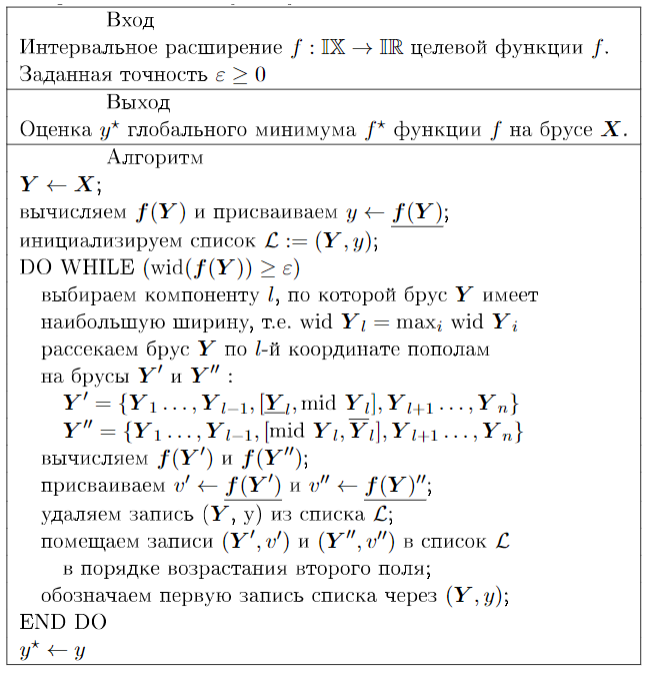
\includegraphics[width=13cm]{glob_opt_image.png}
                \label{fig:Himmel1}
            \end{figure}
            
            
              
	\section{Реализация}
		Лабораторная работа выполнена с помощью встроенных средств языка программирования Python с использованием библиотек matplotlib, intvalpy, numpy в среде разработки Jupyter Notebook. 
		\pagebreak
		
	
	
	\section{Результаты}
        \subsection{Задача линейной регрессии}
	        Для того, чтобы точечная матрица была особенной, достаточно линейной зависимости ее строк. В случае рассматриваемой матрицы (\ref{lin_reg}) это достижимо при $\varepsilon\geq0.05$. Проверим, что при $\varepsilon=0.05$ найдется особенная точечная матрица:
            \begin{equation*}
                \mathbf{X}=\begin{pmatrix}
              [0.9, 1]& 1\\
              [1.1, 1]& 1
            \end{pmatrix},\: X=\begin{pmatrix}
              1.05& 1\\
              0.95& 1
            \end{pmatrix}\in\mathbf{X},\:\det(X)=0
            \end{equation*}

            \begin{figure}[H]
                \centering
                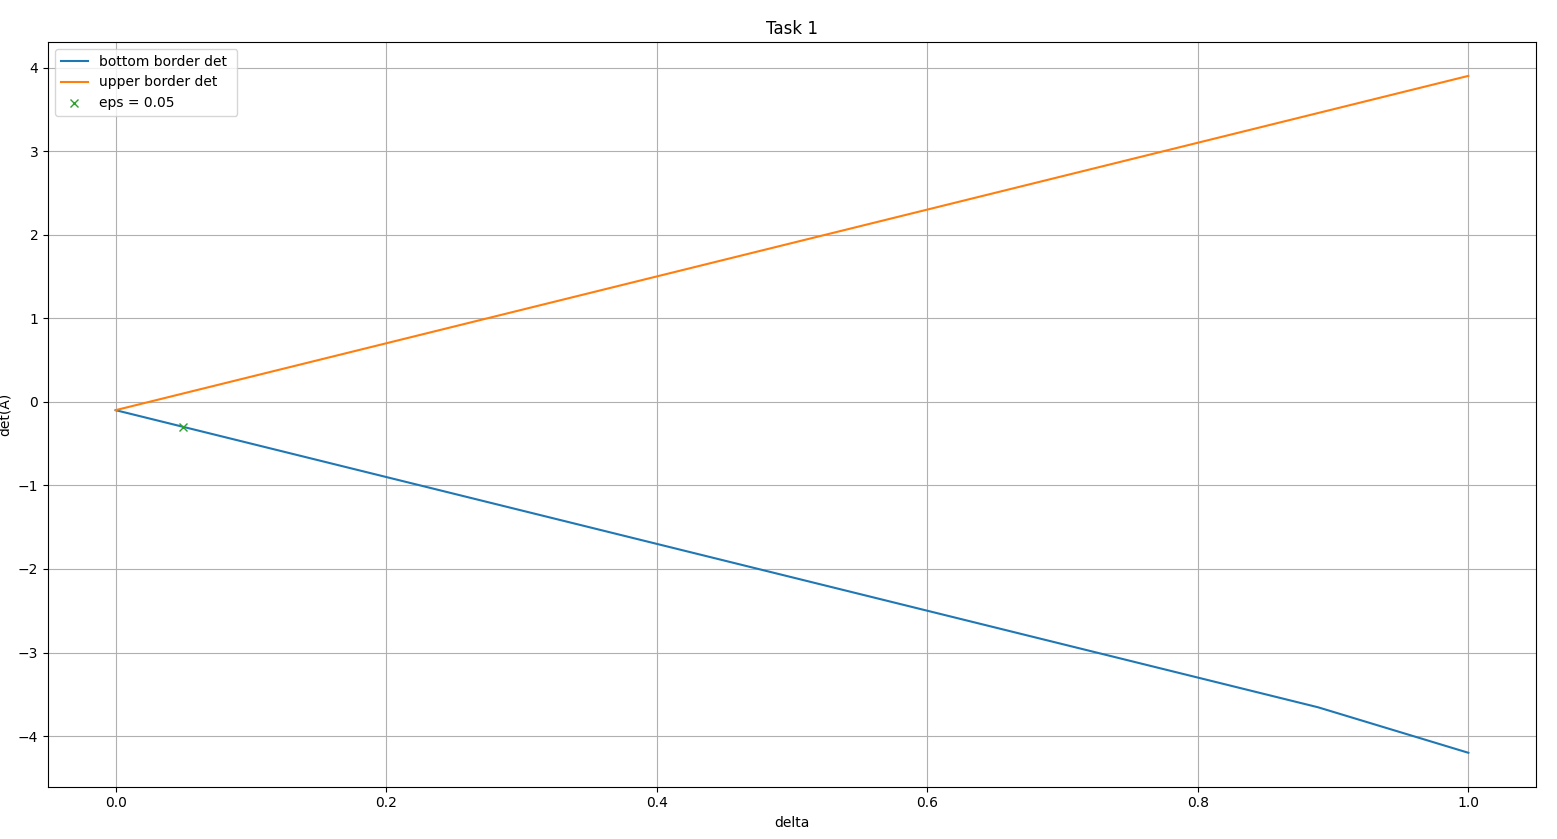
\includegraphics[width=16cm]{eps-0.05.png}
            \end{figure}

            Видим что при $\varepsilon >= 0.05 $ определитель матрицы содержит 0
                
            
            
            
        	
		\subsection{Задача томографии}
    		\subsubsection{Критерий Баумана}
    		    Воспользуемся критерием Баумана
                
                Найдем, при каких значениях $\varepsilon$ матрица является неособенной. Тогда особенной она будет при всех остальных значениях
                \begin{center}
                    \begin{tabular}{ |c|c|c| } 
                         \hline
                         $ \varepsilon$ & особенна матрица \\ 
                         \hline
                         0.00 & Нет \\ 
                         0.01 & Нет \\ 
                         0.02 & Нет \\ 
                         0.03 & Нет \\ 
                         0.04 & Нет \\ 
                         0.05 & Да \\ 
                         0.06 & Да \\ 
                         0.07 & Да \\ 
                         0.08 & Да \\ 
                         \hline
                    \end{tabular}
                \end{center}

                Видим что при $\varepsilon >= 0.05 $ матрица особенна и $\varepsilon < 0.05 $ неособенна.
                
                
    		  
    	\newpage	    
    		    
    		    
	    \subsection{Глобальная оптимизация}
	        \subsubsection{Функция Химмельблау}
    	        Для функции Химмельблау
    	        \begin{equation}\label{Himmel}
                    f(x, y) = (x^2 + y - 11)^2 + (x + y^2 - 7)^2
                \end{equation}
    	        
    	        построим ее график и обозначим глобальные минимумы
    	        
                \begin{equation*}
                    min = 
                     \begin{cases}
                       f(3, 2) = 0 \\
                		f(-2.805118, 3.131312) = 0\\
                		f(-3.779310, -3.283186) = 0\\
                		f(3.584428, -1.848126) = 0\\
                     \end{cases}
                \end{equation*}
    	        
    	        \begin{figure}[H]
                    \centering
                    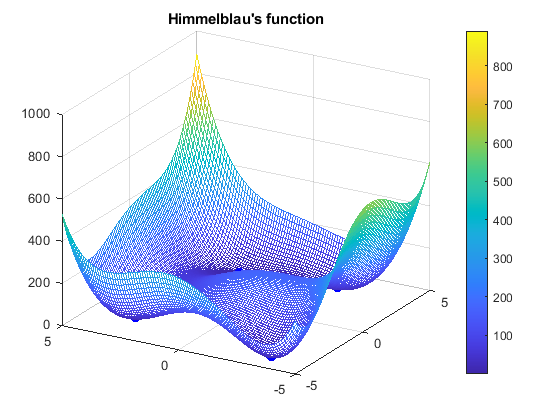
\includegraphics[width=13cm]{Himmablau1.png}
                    \caption{График функции Химмельблау (\ref{Himmel})}
                    \label{fig:Himmel1}
                \end{figure}
                
                \begin{figure}[H]
                    \centering
                    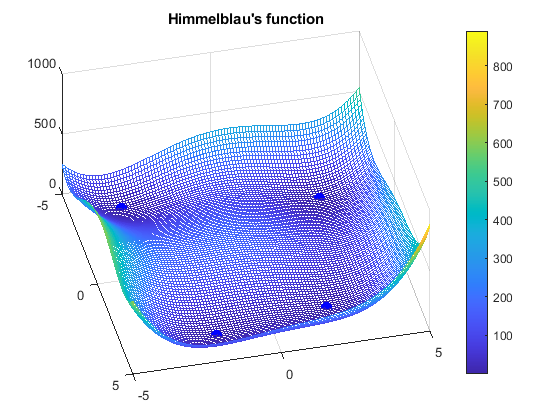
\includegraphics[width=13cm]{Himmablau2.png}
                    \caption{График функции Химмельблау (\ref{Himmel})}
                    \label{fig:Himmel2}
                \end{figure}
    	    
    	        \begin{figure}[H]
                    \centering
                    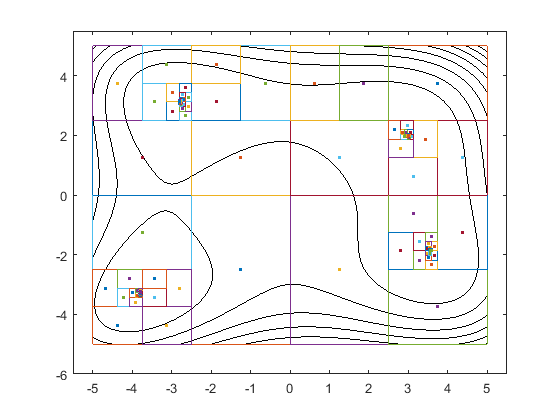
\includegraphics[width=13cm]{Himmablau_vizualization.png}
                    \caption{Визуализация алгорита для функции Химмельблау (\ref{Himmel})} \label{fig:Himmel_vizualization}
                \end{figure}
    	    
    	        Можно видеть, что число брусьев сгущается по мере приближения к каждому из 4 экстремумов

             Найденный алгоритмом глобальный минимум:
             \begin{center}
                    \begin{tabular}{ |c|c|c| } 
                         \hline
                         $ x^*$ & $y^*$ & $f(x^*,y^*)$ \\ 
                         \hline
                         3.58447265625 & -1.8486328125 & 0 \\ 
                         \hline
                    \end{tabular}
                \end{center}
    	        
    	        Также построим еще графики, отображающие радиусы рабочих брусов и сходимость алгоритма (расстояние до ближайшего на каждой итерации экстремума)
    	        
    	        \begin{figure}[H]
                    \centering
                    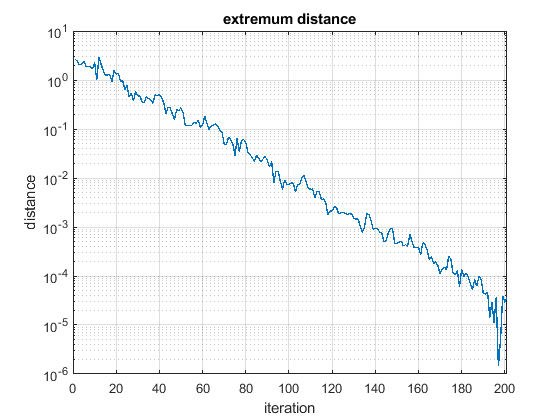
\includegraphics[width=13cm]{Himablau_extr_dist.png}
                    \caption{Расстояние до точки экстремума для функции Химмельблау (\ref{Himmel})} \label{fig:Himmel_vizualization}
                \end{figure}
                
                
                \begin{figure}[H]
                    \centering
                    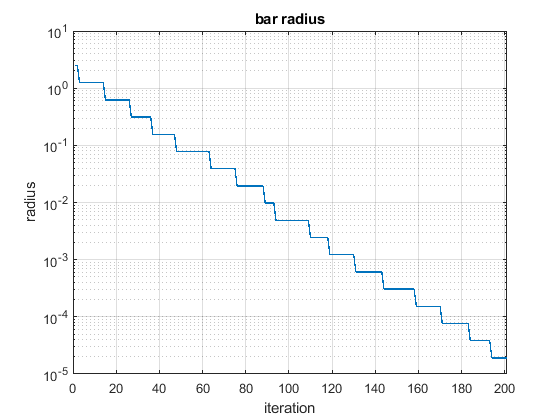
\includegraphics[width=13cm]{Himmel_radius.png}
                    \caption{Радиусы рабочих брусов для функции Химмельблау (\ref{Himmel})} \label{fig:Himmel_radius}
                \end{figure}
            
            \newpage
            
            \subsubsection{Функция Била}
                Для функции Била
                \begin{equation}\label{Booth}
                    f(x, y) = (1.5 - x + xy)^2 + (2.25 - x + xy^2)^2 + 2.625 - x + xy^3)^2
                \end{equation}
                
                также построим ее график и обозначим глобальный минимум
                
                \begin{equation}
                    min = f(3, 0.5) = 0
                \end{equation}
                
                \begin{figure}[H]
                    \centering
                    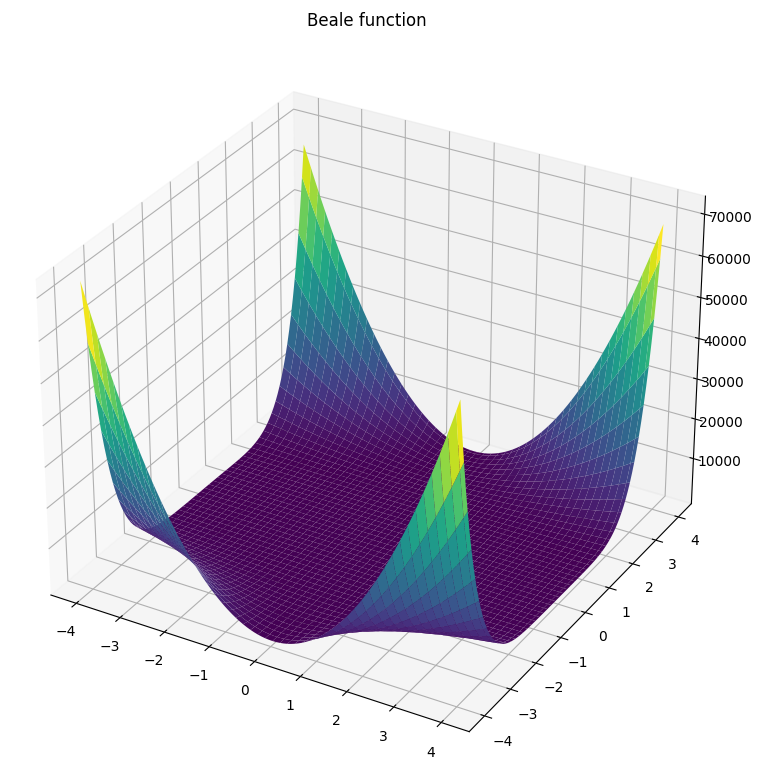
\includegraphics[width=13cm]{beale.png}
                    \caption{График функции Била (\ref{Booth})}
                    \label{fig:Boot1}
                \end{figure}
                
                
                \begin{figure}[H]
                    \centering
                    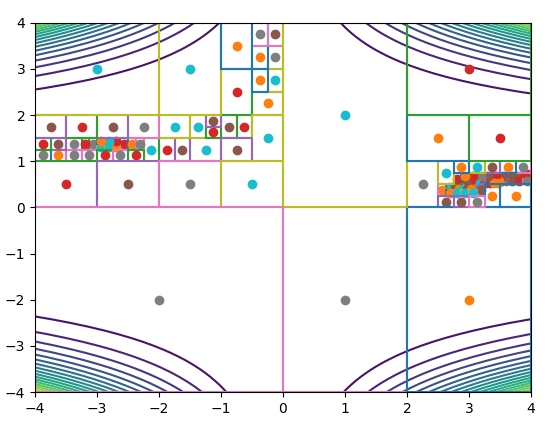
\includegraphics[width=13cm]{beale_visual.png}
                    \caption{Визуализация алгоритма для функции Била (\ref{Booth})}
                    \label{fig:Boot2}
                \end{figure}

                Найденный алгоритмом глобальный минимум:
             \begin{center}
                    \begin{tabular}{ |c|c|c| } 
                         \hline
                         $ x^*$ & $y^*$ & $f(x^*, y^*)$ \\ 
                         \hline
                         2.9951171875 & 0.4999234375 & 0 \\ 
                         \hline
                    \end{tabular}
                \end{center}
                
                Здесь также число брусьев сгущается по мере приближения к экстремуму
                
                \begin{figure}[H]
                    \centering
                    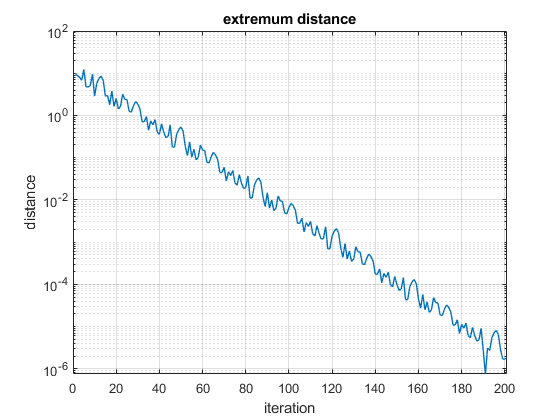
\includegraphics[width=13cm]{Booth_extr_dist.png}
                    \caption{Расстояние до точки экстремума для функции Била (\ref{Booth})}
                    \label{fig:Boot3}
                \end{figure}
                
                
                \begin{figure}[H]
                    \centering
                    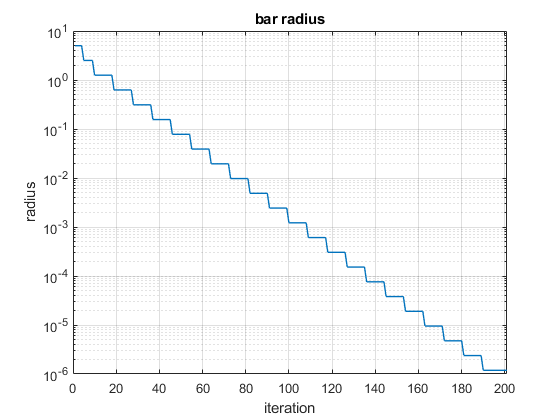
\includegraphics[width=13cm]{Booth_rad.png}
                    \caption{Радиусы рабочих брусов для функции Била (\ref{Booth})}
                    \label{fig:Boot4}
                \end{figure}
                
                
	
	\section{Обсуждение}
	    \begin{enumerate}
    	    \item Что в задачах линейной регресии, что в задачах полиномиальной регрессии мы рассматриваем матрицы $\mathbf{X}_n\in\mathbb{IR}^{n\times n}$. При переходе от задач линейной регрессии к задачам полиномиальной, увеличивается параметр $n$. При этом при достаточной близости $mid\mathbf{X}_n$ друг к другу и высокой неопределенности значений входных паременных матрица может стать неопределенной
    	   
           \item 
           При переходе от задачи (\ref{problem:lin_reg}) к задаче (\ref{problem:tomography}) были введены дополнительные интервальные величины. Например, было две пары точек $(x_1, y_1), (x_2, y_2)$. Составим регрессионую матрицу $X_1$ из $x_1, x_2$ для линейной регрессии. Найдем $\varepsilon$ при котором пересечение интервалов  $\textbf{x}_1$ и $\textbf{x}_2$ непустое, то есть найдем общую точку $x$. Добавим $n-2$ точек пар точек и составим матрицу $X_2$ из $x_1, ... ,x_n$ для многочлена $n-1$ порядка. По основной теореме интервальной арифметики (\ref{main_theorem}) - результать операции над точечным представлением интервала принадлежит результату операции над интервальным представлением. $x^n$ будет принадлежать также и $\textbf{x}_1^n$ и $\textbf{x}_2^n$. В интервальной матрице будет содержаться точечная особая, по первым двум строкам, и интервальная матрица будет особая.
           Следовательно, характер оценки $\varepsilon$ не будет зависеть от добавляемых пар точек. Оценка $\varepsilon$ будет не увеличиваться
           
    
           
           \item На основе графиков можно сказать, метод нахождения глобального экстремума показал монотонное убывание радиусов брусов и довольно точные положения экстремумов, для обеих функций точность около $10^{-5}$
       
       \end{enumerate}
       
       
       \newpage
	    
	    
	\begin{thebibliography}{9} 
		\addcontentsline{toc}{section}{Список литературы}
  
        \bibitem{linear_regression} А.Н. Баженов. Интервальный анализ. Основы теории и учебные примеры. - СПб., 2020.

  
		
		\bibitem{linear_regression} Test functions for optimization, URL: \url{https://en.wikipedia.org/wiki/Test_functions_for_optimization}
		
		
	\end{thebibliography}
        \section{Приложение}
            Код программы на GitHub Url https://github.com/lpvmak/interval
\end{document}